% !TEX root = 00_main_aaai_2027.tex
% Provenance: experiments/archive/13_toy_pearson_vs_ce_nonlinear_ratings_start_10Nov2026_end_10Nov2026 (setup, CE/RPS/Pearson fits);
% experiments/06_toy_rank_and_mixed_correlation_objectives_vs_ce_start_13Nov2026/results.md (rank and mixed objectives);
% experiments/07_toy_optimizer_restarts_and_budget_for_nonconvex_objectives_start_13Nov2026/results.md (optimizer check);
% experiments/08_toy_target_complexity_and_tuned_regularization_vs_ratings_needed_start_14Nov2026/results.md and results/tables.md
% (scenarios C and D, tuned ridge, constant baseline). Figure and the 2,048-task ratios are printed by
% experiments/08_toy_target_complexity_and_tuned_regularization_vs_ratings_needed_start_14Nov2026/scripts/make_paper_figure.py.
\section{Learning a Judge from Sparse Ratings}
\label{sec:learning}
The identification study above selects among fixed candidates.
We now train a flexible judge and ask how many ratings proper-loss training needs before it beats correlation training on held-out data.

\paragraph{Setup.}
Each synthetic task has a feature $x\sim\mathrm{Unif}[-1,1]$ and ratings $R\mid x\sim\mathrm{BetaBin}\big(5,\mu(x)\kappa(x),(1-\mu(x))\kappa(x)\big)$ with mean $5\mu(x)$; a smaller $\kappa$ means more rater disagreement.
Four targets place their information differently.
(A) The mean is nearly constant, $\mu=0.5+0.08x$, while disagreement $\kappa(x)=e^{1.5+2.2\cos(1.5\pi x)}$ varies about 80-fold.
(B) The mean is nonlinear, $\mu=0.1+0.8\big(\tfrac{x+1}{2}\big)^2$, with the same varying disagreement.
(C) B's mean with constant $\kappa=e^{1.5}$.
(D) A linear mean, $\mu=0.5+0.35x$, with constant $\kappa=e^{1.5}$; this is the case most favorable to correlation.
The judge is a softmax over the six ratings of a linear map of 13 cosine and sine features of $x$.
It is trained on $n$ tasks with three ratings each by CE, by RPS, or by Pearson correlation between its expected rating and each task's mean rating.
In A and B we also train with smooth surrogates of Spearman and Kendall correlation and an equal Pearson--Spearman mix.
All fits use the ridge penalty $\frac{1}{n}\|W\|^2$ and L-BFGS-B started at the training rating histogram; we also tune the ridge strength by four-fold cross-validation over the training tasks.
Each judge is scored on 500 fresh tasks against the true distribution, with 100 seeds per size and paired 95\% bootstrap intervals over seeds.
Procedures and predictions were committed before measurement.

\begin{figure}[t]
\centering
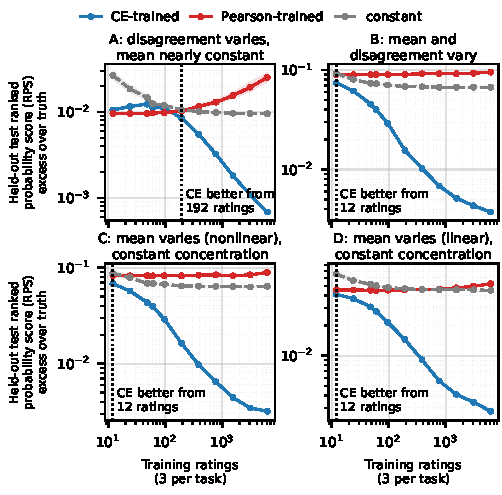
\includegraphics[width=\columnwidth]{figures/fig_ratings_needed.pdf}
\caption{\textbf{Ratings needed before proper-loss training wins.} Held-out test RPS excess over the true distribution (log scale; lower is better) against training ratings, for judges trained by CE or by Pearson correlation and for a constant training-histogram forecast, in four synthetic targets. Dotted lines mark the size from which the CE-trained judge is significantly better at every larger size (paired 95\% bootstrap over 100 seeds). Judges are fitted by L-BFGS-B with ridge $\frac{1}{n}\|W\|^2$; CE is convex in $W$, Pearson is not.}
\label{fig:ratings}
\end{figure}

\paragraph{Results.}
Wherever the mean carries information (B, C and D, including the linear case), the CE-trained judge has significantly lower held-out RPS than the Pearson-trained judge at every size from 12 ratings (Figure~\ref{fig:ratings}).
Correlation training wins only in A, where the mean is nearly constant: up to 96 ratings, with CE better from 192.
Rank and mixed correlation objectives do no better; at 2,048 tasks their held-out RPS excess is 9--26 times the CE-trained judge's in B and 37--46 times in A.
At large sizes the Pearson-trained judge's held-out RPS is worse than the constant forecast's in every target, while its correlation with the true mean reaches 0.85--0.99.
Even on correlation, the CE-trained judge's held-out correlation with the true mean is never significantly lower until the Pearson-trained judge overtakes, from 1,536 ratings in B and C and 3,072 in D, and never in A.

Two checks support these results.
First, the correlation objectives are not convex, and their fits rarely converge: no Pearson fit with 32 or more tasks converged within 400 iterations.
Refitting with five times the budget and the best of five starts (30 seeds, up to 1,024 tasks) usually improved the training correlation but left every held-out RPS crossover unchanged.
Second, tuning the ridge on validation data moved A's crossover to 96 ratings, but the choice was noisy with 16 or fewer training tasks.

\paragraph{Interpretation.}
Correlation training helps at small sample sizes only when the target's structure lies in higher moments that few ratings cannot pin down and its mean carries little signal.
Matching the mean while keeping the average spread is then the best early strategy.
Where the mean is informative, the loss-trained judge learns it at least as fast.
The ratings needed therefore depend on where the target's information lies, not on its complexity alone: B is as complex as A but needs 12 ratings.
These results use one input feature and one judge family; which regime human ratings occupy is open.
